% \documentclass[sigplan,10pt,anonymous,review]{acmart}\settopmatter{printfolios=true,printccs=false,printacmref=false}
\documentclass[runningheads]{llncs}

\usepackage[T1]{fontenc}
\usepackage[utf8]{inputenc}
\usepackage{microtype} % Better typesetting for PDFs -- is enabling this ok?
\usepackage{balance}

\usepackage{amsmath}
\usepackage{amssymb}
% \usepackage{amsthm}

%\usepackage{eufrak} %The eufrak package is redundant if the amsfonts package is used
\usepackage{mathpartir}
\DeclareMathAlphabet{\mathpzc}{OT1}{pzc}{m}{it}
\usepackage[boxed]{algorithm}
\usepackage{enumerate}
\usepackage{cprotect}

\usepackage[numbers]{natbib}

\usepackage{listings}
\usepackage{lstautogobble}
\usepackage{graphicx}
\usepackage{tabularx}
\usepackage{booktabs}
\usepackage{ragged2e}  % for '\RaggedRight' macro (allows hyphenation)
\usepackage{color}
\usepackage[noend]{algpseudocode}
\usepackage{caption}
\usepackage[font=scriptsize]{subcaption}
\usepackage{hyperref}
\usepackage{float}
\usepackage{wrapfig}

\usepackage{multirow}
\usepackage{siunitx}

\usepackage{tikz}
\usetikzlibrary{positioning,fit,shadows,decorations, arrows, shapes, decorations.markings,decorations.pathmorphing,calc}

\usepackage{pgfplots}


\tikzset{
  -|-/.style={
    to path={
      (\tikztostart) -| ($(\tikztostart)!#1!(\tikztotarget)$) |- (\tikztotarget)
      \tikztonodes
    }
  },
  -|-/.default=0.5,
  |-|/.style={
    to path={
      (\tikztostart) |- ($(\tikztostart)!#1!(\tikztotarget)$) -| (\tikztotarget)
      \tikztonodes
    }
  },
  |-|/.default=0.5,
}

\clubpenalty = 10000
\widowpenalty = 10000
\displaywidowpenalty = 10000

% Not really meant for highlighting isabelle source, but for easily writing latex that looks like
% isabelle
% 
% keyword level 1 - isabelle outer syntax 
% keyword level 2 - isabelle inner syntax programming constructs (if, let, etc)
% keyword level 3 - standard constants (length, mod, etc)
% keyword level 4 - isabelle proof methods


% \newcommand{\lsem}{\ensuremath{\mathopen{[\![}}}
% \newcommand{\rsem}{\ensuremath{\mathclose{]\!]}}}

\lstdefinelanguage{isabelle}{
  morekeywords={theorem,theorems,corollary,lemma,lemmas,locale,begin,end,fixes,assumes,shows,and,class,
    constrains , definition, where, apply, done,unfolding, primrec, fun, using, by, for, uses,
    schematic_lemma, concrete_definition, prepare_code_thms, export_code, datatype, type_synonym, typedef, value,
    proof, next, qed, show, have, hence, thus, interpretation, fix, context, sepref_definition,is
 } ,
  morekeywords=[2]{rec, return, bind, foreach, if, then, else, do, let, in, res, spec, fail, assert, while, case, of,
    check},
%  morekeywords=[3]{length,mod,insert},
%   morekeywords=[4]{simp,auto,intro,elim,rprems,refine_mono,refine_rcg},
  sensitive=True,
  morecomment=[s]{(\*}{\*)},
}

\lstset{
    language=isabelle,
    mathescape=true,
    escapeinside={--"}{"},
    basicstyle={\itshape},
    keywordstyle=\rm\bfseries,
    keywordstyle=[2]\rm\tt,
    keywordstyle=[3]\rm,
    keywordstyle=[4]\rm,
    showstringspaces=false,
    keepspaces=true,
    columns=[c]fullflexible}
\lstset{literate=
  {"}{}0
  {'}{{${}^\prime\!$}}1
  {\%}{{$\lambda$}}1
  {\\\%}{{$\lambda$}}1
  {\\\$}{{$\mathbin{\,\$\,}$}}1
  {->}{{$\rightarrow$}}1
  {<-}{{$\leftarrow$}}1
  {<.}{{$\langle$}}1
  {.>}{{$\rangle$}}1
  {<=}{{$\le$}}1
  {>=}{{$\ge$}}1
  {<->}{{$\leftrightarrow$}}1
  {-->}{{$\longrightarrow$}}2
  {<-->}{{$\longleftrightarrow$}}1
  {=>}{{$\Rightarrow$}}1
  {==}{{$\equiv$}}2
  {==>}{{$\implies$}}2
  {<=>}{{$\Leftrightarrow$}}1
  {~=}{{$\ne$}}1
  {|}{{$\mid$}}1
  {-`}{{$\rightharpoonup$}}1
  {|`}{{$\restriction$}}1
  {!!}{{$\bigwedge$}}1
  {(}{{$($}}1
  {)}{{$)$}}1
  {\{}{{$\{$}}1
  {\}}{{$\}$}}1
  {[}{{$[$}}1
  {]}{{$]$}}1
  {[|}{{$\llbracket$}}1
  {|]}{{$\rrbracket$}}1
  {\\<lbrakk>}{{$\lsem$}}1
  {\\<rbrakk>}{{$\rsem$}}1
  {|-}{{$\vdash$}}1
  {|=}{{$\models$}}1
  {|->}{{$\mapsto$}}1
  {|_|}{{$\bigsqcup$}}1
  {...}{{$\dots$}}1
  {\\x}{{$\times$}}1
  {_0}{{${}_0$}}1
  {_1}{{${}_1$}}1
  {_2}{{${}_2$}}1
  {_3}{{${}_3$}}1
  {_4}{{${}_4$}}1
  {_5}{{${}_5$}}1
  {_6}{{${}_6$}}1
  {_7}{{${}_7$}}1
  {_8}{{${}_8$}}1
  {_9}{{${}_9$}}1
  {_L}{{${}_L$}}1
  {\\_n}{{${}_n$}}1
  {\\_i}{{${}_i$}}1
  {\\_j}{{${}_j$}}1
  {\\_x}{{${}_x$}}1
  {\\_y}{{${}_y$}}1
  {\\impl}{{${}_\dagger$}}1
  {^*}{{$^*$}}1
  {^k}{{$^k$}}1
  {^d}{{$^d$}}1
  {\\<^sup>*}{{$^*$}}1
  {\\<^sub>*}{{$_*$}}1
  {\\<^sub>A}{{$_A$}}1
  {\\<^sub>r}{{$_r$}}1
  {\\<^sub>a}{{$_a$}}1
  {:_i}{{$:_i$}}1
  {\\<A>}{{$\mathcal{A}$}}1
  {\\<O>}{{\sf o}}1
  {\\<Phi>}{{$\Phi$}}1
  {\\<Psi>}{{$\Psi$}}1
  {\\<sigma>}{{$\sigma$}}1
  {\\<cdot>}{{$\cdot$}}1
  {\\<in>}{{$\in$}}1
  {\\<le>}{{$\le$}}1
  {\\<noteq>}{{$\ne$}}1
  {\\<lambda>}{{$\lambda$}}1
  {\\<longrightarrow>}{{$\longrightarrow$}}1
  {\\<longleftrightarrow>}{{$\longleftrightarrow$}}1
  {\\<Rightarrow>}{{$\Rightarrow$}}1
  {\\<Longrightarrow>}{{$\Longrightarrow$}}1
  {\\<rightarrow>}{{$\rightarrow$}}1
  {\\<leftarrow>}{{$\leftarrow$}}1
  {\\<mapsto>}{{$\mapsto$}}1
  {\\<equiv>}{{$\equiv$}}1
  {\\<and>}{{$\and$}}1
  {\\<or>}{{$\vee$}}1
  {\\<And>}{{$\bigwedge$}}1
  {\\<Up>}{{$\Uparrow$}}1
  {\\<Down>}{{$\Downarrow$}}1
  {\\<Union>}{{$\bigcup$}}1
  {\\<up>}{{$\uparrow$}}1
  {\\<down>}{{$\downarrow$}}1
  {\\<times>}{{$\times$}}1
  {\\<forall>}{{$\forall$}}1
  {\\<exists>}{{$\exists$}}1
  {\\<nexists>}{{$\nexists$}}1
  {\\<union>}{{$\cup$}}1
  {\\<inter>}{{$\cap$}}1
  {\\<subset>}{{$\subset$}}1
  {\\<subseteq>}{{$\subseteq$}}1
  {\\<supset>}{{$\supset$}}1
  {\\<supseteq>}{{$\supseteq$}}1
  {\\<alpha>}{{$\alpha$}}1
  {\\<beta>}{{$\beta$}}1
  {\\<gamma>}{{$\gamma$}}1
  {\\alpha}{{$\alpha$}}1
  {\\beta}{{$\beta$}}1
  {\\gamma}{{$\gamma$}}1
  {\\<Gamma>}{{$\Gamma$}}1
  {\\<langle>}{{$\langle$}}1
  {\\<rangle>}{{$\rangle$}}1
  {\\<not>}{{$\neg$}}1
  {\\<box>}{{$\oblong$}}1
  {\\<bot>}{{$\bot$}}1
  {\\<top>}{{$\top$}}1
  {\\<notin>}{{$\notin$}}1
  {\\<guillemotright>}{{$\gg$}}1
  {\\in}{$\in$}1
  {\\and}{$\wedge$}1
  {\\or}{$\vee$}1
  {\\Phi}{{$\Phi$}}1
  {\\Psi}{{$\Psi$}}1
  {\\le}{{$\le$}}1
  {\\Up}{{$\Uparrow$}}1
  {\\Down}{{$\Down$}}1
  {>>}{{$\gg$}}1
  {>>=}{{${\gg}{=}$}}1
  {<*lex*>}{{$\times_{\sf lex}$}}1
  {\\<open>}{{\rm\guilsinglleft}}1
  {\\<close>}{{\rm\guilsinglright}}1
}

% \newcommand{\is}{\lstinline[language=isabelle,basicstyle=\normalsize\ttfamily\slshape]}
\newcommand{\is}{\lstinline[language=isabelle]}
\newcommand{\q}[1]{\mbox{\guilsinglleft{#1}\hspace{-2.5pt}\guilsinglright}}
% \newcommand{\isai}[1]{\q{\lstinline[language=isabelle,basicstyle=\normalsize\ttfamily\slshape]{#1}}}
\cMakeRobust\q

\lstset{captionpos=b}
\lstset{numberbychapter=false}
\lstset{autogobble}


\newcolumntype{Y}{>{\RaggedRight\arraybackslash}X} % Multiline column, automatic width




  \newcommand{\false}{\textrm{false}}
  \newcommand{\true}{\textrm{true}}



% \theoremstyle{definition}
% \newtheorem{example}{Example}[section]

% \overfullrule=8pt


\begin{document}

\title{Efficient Verified Implementation of Introsort and Pdqsort}


\author{Peter Lammich}
\institute{The University of Manchester, UK}
% \email{peter.lammich@machester.ac.uk}
%
% \authorinfo{Peter Lammich}
%            {The University of Manchester, UK}
%            {peter.lammich@machester.ac.uk}

\maketitle



\begin{abstract}
  Sorting algorithms are an important part of most standard libraries, and
  both, their correctness and efficiency is crucial for many applications.

  As generic sorting algorithm, the GNU C++ Standard Library implements the Introsort algorithm,
  a combination of quicksort, heapsort, and insertion sort. The Boost C++ Libraries implement Pdqsort,
  an extension of Introsort that achieves linear runtime on inputs with certain patterns.

  We verify Introsort and Pdqsort in the Isabelle LLVM verification framework,
  closely following the state-of-the-art implementations from GNU and Boost.
  On an extensive benchmark set, our verified implementations perform on par with the originals.
\end{abstract}


% \category{F.3.1}{Logics and Meanings of Programs}{Specifying and Verifying and Reasoning about Programs}

% general terms are not compulsory anymore,
% you may leave them out
% \terms Verification
% term1, term2

% \keywords
% Sorting, Interactive Theorem Proving, Isabelle HOL, Stepwise Refinement, Separation Logic, LLVM


\section{Introduction}
%   In this paper, we present verified and efficient implementations of
%   Musser's introspective sorting algorithm (Introsort)~\cite{Muss97} and its
%   extension \emph{Pattern-Defeating Quicksort} (Pdqsort)~\cite{pdqsort}.
%   Using the Isabelle Refinement Framework with its LLVM backend~\cite{La19-llvm},
%   we closely follow the implementations of Introsort and Pdqsort from
%   the GNU C++ Library (libstdc++)~\cite{libstdc++} and the Boost C++ Libraries~\cite{boost}.
%   The resulting sorting algorithms
%   are verified down to their representation in the LLVM intermediate language~\cite{LLVM-manual},
%   and perform on-par with the unverified original implementations on an extensive set of benchmarks.

  Sorting algorithms are an important part of any standard library.
  The GNU C++ Library (libstdc++)~\cite{libstdc++} implements Musser's introspective sorting algorithm (Introsort)~\cite{Muss97}.
  It is a combination of quicksort, heapsort, and insertion sort,
  which has the fast average case runtime of quicksort and the optimal $O(n\log(n))$
  worst-case runtime of heapsort.
  The Boost C++ Libraries~\cite{boost} provide a state-of-the-art implementation of
  \emph{Pattern-Defeating Quicksort} (Pdqsort)~\cite{pdqsort}, an extension of Introsort to
  achieve better performance on inputs that contain certain patterns like already sorted sequences.
  Verification of these algorithms and their state-of-the-art implementations is far from trivial,
  but turns out to be manageable when handled with adequate tools.

  Sorting algorithms in standard libraries have not always been correct.
  The Timsort~\cite{Peters02} algorithm in the Java standard library has a history of bugs\footnote{see \url{https://bugs.java.com/bugdatabase/view_bug.do?bug_id=8011944}}, the (hopefully) last of which was only found by a formal verification effort~\cite{GRBBH15}.
  Also, many real-world mergesort implementations suffered from an overflow bug~\cite{bs_flaw_blogpost}.
  Finally, LLVM's libc++~\cite{libc++} implements a different quicksort based sorting algorithm. While it may be functionally correct,
  it definitely violates the C++ standard by having a quadratic worst-case run time\footnote{See~\url{https://bugs.llvm.org/show_bug.cgi?id=20837}. This has not been fixed by January 2020.}.

  In this paper, we present efficient implementations of Introsort and Pdqsort that are verified down to their
  LLVM intermediate representation~\cite{LLVM-manual}. The verification uses the
  Isabelle Refinement Framework~\cite{LaTu12}, and its recent Isabelle-LLVM backend~\cite{La19-llvm}.
  We also report on two extensions of Isabelle-LLVM, to handle nested container data structures and to automatically
  generate C-header files to interface the generated code. Thanks to the modularity of the Isabelle Refinement Framework,
  our verified algorithms can easily be reused in larger verification projects.

  While sorting algorithms are a standard benchmark for theorem provers and program verification tools,
  verified real-world implementations seem to be rare: apart from our work, we are only aware of
  two verified sorting algorithms~\cite{GRBBH15,BSSU17} from the Java standard library.

  The complete Isabelle/HOL formalization and the benchmarks are available at \url{http://www21.in.tum.de/~lammich/isabelle_llvm/}.


%
%
%   Mention implementation in libc++, but not standard-conformant! $O(n^2)$ worst case
%
%   The Isabelle LLVM verification framework
%     stepwise refinement, code export to LLVM
%
%   Contributions
%     D First verified introsort? (that is on-par with state-of-the art implementation!)
%     D Case-Study: Verification of state-of-the art implementations of medium-complex algorithms possible!
%     ! Prototype for handling nested container data structures.




\section{The Introsort and Pdqsort Algorithms}
  The Introsort algorithm by Musser~\cite{Muss97} is a generic unstable sorting algorithm
  that combines the good average-case runtime of quicksort~\cite{Hoare61} with the optimal $O(n\log(n))$ worst-case complexity of heapsort~\cite{Will64}.
  The basic idea is to use quicksort as main sorting algorithm, insertion sort for small partitions, and heapsort when the recursion
  depth exceeds a given limit, usually $2\lfloor\log_2 n\rfloor$ for $n$ elements.


  \begin{algorithm}
  \begin{algorithmic}[1]
    \Procedure{introsort}{$xs,l,h$}
      \If{$h-l>1$} \label{l:intrs:trivial}
        \State{\Call{introsort\_aux}{$xs,l,h,2\lfloor\log_2(h-l)\rfloor$}} \label{l:intrs:aux}
        \State{\Call{final\_insort}{$xs,l,h$}} \label{l:intrs:finalis}
      \EndIf
    \EndProcedure

    \Procedure{introsort\_aux}{$xs,l,h,d$}
      \If{$h-l>\textrm{threshold}$} \label{l:intrs:threshold}
        \If{$d=0$}~\Call{heapsort}{$xs,l,h$} \label{l:intrs:heapsort}
        \Else
          \State{$m\gets\Call{partition\_pivot}{xs,l,h}$} \label{l:intrs:part}
          \State{\Call{introsort\_aux}{$xs,l,m,d-1$}}  \label{l:intrs:rec1}
          \State{\Call{introsort\_aux}{$xs,m,h,d-1$}}  \label{l:intrs:rec2}
        \EndIf
      \EndIf
    \EndProcedure
  \end{algorithmic}
  \caption{Introsort}\label{alg:introsort}
  \end{algorithm}



  Algorithm~\ref{alg:introsort} shows our implementation of Introsort, which closely follows the implementation in libstdc++~\cite{libstdc++}.
  The function \textsc{introsort} sorts the slice \is$l..<h$ of the list\footnote{%
    Our formalization initially uses lists to represent the sequence of elements to be sorted, and refines them to arrays later (cf.\ Sec.\ \ref{sec:imp_impl}).
  } $xs$.
  If there is more than one element (line~\ref{l:intrs:trivial}), it initializes a depth
  counter and calls the function \textsc{introsort\_aux} (line~\ref{l:intrs:aux}), which partially sorts the list such that every element is no more than
  threshold positions away from its final position in the sorted list. The remaining sorting is then done by insertion sort (line~\ref{l:intrs:finalis}).
  The function \textsc{introsort\_aux} implements a recursive quicksort scheme: recursion stops if the slice becomes smaller than the the threshold (line~\ref{l:intrs:threshold}).
  If the maximum recursion depth is exhausted, heapsort is used to sort the slice (line~\ref{l:intrs:heapsort}).
  Otherwise, the slice is partitioned (line~\ref{l:intrs:part}), and the procedure is
  recursively invoked for the two partitions (line~\ref{l:intrs:rec1}--\ref{l:intrs:rec2}).

  Note that we do not try to invent our own implementation, but closely follow the existing (and hopefully well-thought) libstdc++ implementation.
  This includes the slightly idiosyncratic partitioning scheme, which leaves the pivot-element as first element of the left partition.
  Moreover, the libstdc++ implementation contains a manual tail-call optimization, replacing the recursive call in line~\ref{l:intrs:rec2} by a loop.
  While we could easily add this optimization in an additional refinement step, it turned out to be unnecessary, as LLVM recognizes and
  eliminates this tail call automatically.

  \begin{algorithm}
  \begin{algorithmic}[1]
    \Procedure{pdqsort}{$lm,xs,l,h,d$}
      \If{$h-l>1$}~\Call{pdqsort\_aux}{$\true,xs,l,h,\log(h-l)$}\EndIf \label{l:pdq:aux}
    \EndProcedure

    \Procedure{pdqsort\_aux}{$lm,xs,l,h,d$}
      \If{$h-l<\textrm{threshold}$}~\Call{insort}{$lm,xs,l,h$} \label{l:pdq:threshold}
      \Else
        \State{\Call{pivot\_to\_front}{$xs,l,h$}} \label{l:pdq:pivotfront}
        \If{$\neg lm \wedge xs[l-1] \not< xs[l]$} \label{l:pdq:eqopt}
          \State{$m\gets \Call{partition\_left}{xs,l,h}$} \label{l:pdq:partleft}
          \State{\textbf{assert} $m+1\le h$} \label{l:pdq:assert}
          \State{\Call{pdqsort\_aux}{$\false,xs,m+1,h,d$}} \label{l:pdq:recright}
        \Else
          \State{$(m,ap)\gets\Call{partition\_right}{xs,l,h}$} \label{l:pdq:part}
          \If{$m-l < \lfloor(h-l)/8\rfloor \vee h-m-1 < \lfloor(h-l)/8\rfloor$} \label{l:pdq:unbal}
            \If{${-}{-}d = 0$}~\Call{heapsort}{xs,l,h};~\Return\EndIf \label{l:pdq:heapsort}
            \State{\Call{shuffle}{xs,l,h,m}} \label{l:pdq:shuffle}
          \ElsIf{$ap \wedge \Call{maybe\_sort}{xs,l,m} \wedge \Call{maybe\_sort}{xs,m+1,h}$}\State{\Return} \label{l:pdq:maybe}
          \EndIf
          \State{\Call{pdqsort\_aux}{$lm,xs,l,m,d$}}        \label{l:pdq:rec1}
          \State{\Call{pdqsort\_aux}{$\false,xs,m+1,h,d$}}  \label{l:pdq:rec2}
        \EndIf
      \EndIf
    \EndProcedure
  \end{algorithmic}
  \caption{Pdqsort}\label{alg:pdqsort}
  \end{algorithm}

  Algorithm~\ref{alg:pdqsort} shows our implementation of Pdqsort.
  As for Introsort, the wrapper \textsc{pdqsort} just initializes a depth counter, and then calls the function \textsc{pdqsort\_aux}
  (line~\ref{l:pdq:aux}),
  which, in contrast to Introsort, completely sorts the list, such that no final insertion sort is necessary.
  Again, the \textsc{pdqsort\_aux} function implements a recursive quicksort scheme, however, with a few additional optimizations.
  Slices smaller than the threshold are sorted with insertion sort (line~\ref{l:pdq:threshold}). If the current slice is not the leftmost one
  of the list, as indicated by the parameter $lm$,
  the element before the start of the slice is guaranteed to be smaller than any element of the slice itself. This can be exploited to omit a comparison
  in the inner loop of insertion sort (cf.~Sec.~\ref{sec:insort}).
  If the slice is not smaller than the threshold, a pivot element is selected and moved to the front of the slice (line~\ref{l:pdq:pivotfront}).
  If the pivot is equal to the element before the current slice (line~\ref{l:pdq:eqopt}), this indicates a lot of equal elements.
  The \textsc{partition\_left} function (line~\ref{l:pdq:partleft}) will put them in the left partition, and then only the right partition needs
  to be sorted recursively (line~\ref{l:pdq:recright}).
  Otherwise, \textsc{partition\_right} (line~\ref{l:pdq:part}) places elements equal to the pivot in the right partition.
  Additionally, it returns a flag $ap$ that indicates that the slice was already partitioned.
  Next, we check for a highly unbalanced partitioning (line~\ref{l:pdq:unbal}), i.e., if one partition is less than 1/8th of the overall size.
  After encountering a certain number of highly unbalanced partitionings, Pdqsort switches to heapsort (line~\ref{l:pdq:heapsort}).
  Otherwise, it will shuffle some elements in both partitions, trying to break up patterns in the input (line~\ref{l:pdq:shuffle}).
  If the input was already partitioned wrt.\ the selected pivot (indicated by the flag $ap$),
  Pdqsort will optimistically try to sort both partitions with insertion sort (line~\ref{l:pdq:maybe}).
  However, these insertion sorts abort if they cannot sort the list with a small number of swaps, limiting the penalty for being too optimistic.
  Finally, the two partitions are recursively sorted (lines~\ref{l:pdq:rec1}--\ref{l:pdq:rec2}).

  Our implementation of Pdqsort closely follows the implementation we found in Boost~\cite{boost}.
  Again, we omitted a manual tail call optimization that LLVM does automatically.
  Moreover, for certain comparison functions, Boost's Pdqsort uses a special branch-aware partitioning algorithm~\cite{EdWe16}.
  We leave its verification to future work, but note that it will easily integrate in our existing formalization.

  While Introsort and Pdqsort are based on the same idea, this presentation focuses on the more complex Pdqsort:
  apart from the more involved \textsc{pdqsort\_aux} function,
  \textsc{pivot\_to\_front} uses Tukey's 'ninther' pivot selection~\cite{Bent93}, while Introsort uses the simpler median-of-three scheme.
  It has two partitioning algorithms used in different situations, and the \textsc{partition\_right} algorithm also
  checks for already partitioned slices. Finally, with \textsc{insort} and \textsc{maybe\_sort}, it uses two different
  versions of insertion sort.


  \section{Verification}
  We use the Isabelle Refinement Framework~\cite{LaTu12,La19-llvm} to formally verify our algorithms.
  It provides tools to develop algorithms by stepwise refinement, and generates code in the LLVM intermediate representation~\cite{LLVM-manual}.

  A program returns an element of the following datatype:
  \begin{lstlisting}
    \<alpha> nres == fail | spec (\<alpha> => bool)
  \end{lstlisting}
  Here \is{fail} represents possible non-termination or assertion violation, and \is{spec P}
  a result nondeterministically chosen to satisfy predicate $P$. Note that we use \is{==} to indicate defining equations.
  We define a \emph{refinement ordering} on \is{nres} by
  \begin{lstlisting}
    spec P <= spec Q == \<forall>x. P x ==> Q x         fail $\not\le$ spec Q          m <= fail
  \end{lstlisting}
  Intuitively, \is{m_1 <= m_2} means
  that \is{m_1} returns fewer possible results than \is{m_2}, and may only fail if \is{m_2} may fail.
  Note that \is$<=$ is a complete lattice, with top element \is$fail$.
  The \emph{monad combinators} are then defined as
  \begin{lstlisting}
    return x == spec y. y=x
    bind (spec P) f == |_|{f x | P x}         bind fail f == fail
  \end{lstlisting}
  Here, \is{return x} deterministically returns \is{x}, and \is{bind m f} chooses a result of \is$m$ and then applies
  \is$f$ to it. If \is$m$ may fail, then the bind may also fail.
  We write \is{ x<-m; f x} for \is{bind m (\<lambda>x. f x)}, and \is{m_1; m_2} for \is{bind m_1 (\<lambda>_. m_2)}.

%   Programs are expressed in the following nondeterminism-error monad.
%   \begin{lstlisting}
%     \<alpha> nres == fail | spec (\<alpha> => bool)                return x == spec y. y=x
%     bind fail f == fail | bind (spec P) f = |_|{f x | P x}
%   \end{lstlisting}
%   Here \is{fail} represents possible non-termination or assertion violation, and \is{spec P}
%   a result nondeterministically chosen to satisfy predicate $P$.
%   We define a \emph{refinement ordering} on \is{nres} by
%   \begin{lstlisting}
%     spec P <= spec Q == \<forall>x. P x --> Q x         fail $\not\le$ spec Q          m <= fail
%   \end{lstlisting}
%   Intuitively, \is{m_1 <= m_2} means
%   that \is{m_1} returns fewer possible results than \is{m_2}, and may only fail if \is{m_2} may fail.
%   Note that \is$<=$ is a complete lattice, with top element \is$fail$.
%   The program \is{return x} returns exactly the value \is{x}.
%   The program \is{bind m f} chooses a result of \is$m$ and then applies \is$f$ to it. If \is$m$ may fail, then the bind may also fail.
%   We will write \is{ x<-m; f x} for \is{bind m (\<lambda>x. f x)}, and \is{m_1; m_2} for \is{bind m_1 (\<lambda>_. m_2)}.

  Arbitrary recursive programs can be defined via a fixed-point construction~\cite{Kr10}.
  An \emph{assertion} fails if its condition is not met, otherwise it returns the unit value:
  \begin{lstlisting}
    assert P == if P then return () else fail;
  \end{lstlisting}
  Assertions are used to express that a program \is{m} satisfies the Hoare triple with
  precondition \is$P$ and postcondition \is$Q$:
  \begin{lstlisting}
    m <= assert P; spec x. Q x
  \end{lstlisting}
  If the precondition is false, the right hand side is \is{fail}, and the statement trivially holds.
  Otherwise, $m$ cannot fail, and every possible result $x$ of $m$ must satisfy $Q$.

  While the Isabelle Refinement Framework provides some syntax to express programs, for better
  readability, we use the slightly more informal syntax that we have already used in Algorithms~\ref{alg:introsort} and \ref{alg:pdqsort}.
  In particular, we treat lists as if they were updated in place, while our actual formalization is purely functional, i.e., generates a new
  version of the list on each update, which is explicitly threaded through the program. Destructively updated arrays will only be introduced in a
  later refinement step (cf.~Sec.~\ref{sec:imp_impl}).

  \subsection{Specification of Sorting Algorithms}\label{sec:sortspec}
  The first step to verify a sorting algorithm is to specify the desired result.
  We specify a sorting algorithm as follows:
  \begin{lstlisting}
    sort_spec xs l h
      == assert l<=h \<and> h<=|xs|; spec xs'. xs =$_{l,h}$ xs' \<and> sorted (xs'[l..<h])
  \end{lstlisting}
%     xs =$_{l,h}$ xs'
%       == xs[0..<l]=xs'[0..<l] \<and> mset (xs[l..<h]) = mset (xs'[l..<h]) \<and> xs[h..]=xs'[h..]
  here \is$|xs|$ is the length of the list \is{xs} and
  \is{xs[I]} is the slice of the list \is{xs} for indexes in the interval \is{I}.
%   and \is{xs[l..]} is short for \is{xs[l..<|xs|${}$]}.
  The equivalence relation \is{xs =$_{l,h}$ xs'} relates lists $xs$ and $xs'$ iff they are equal outside the slice \is$l..<h$
  and $xs$ is a permutation of $xs'$.
  To simplify the presentation, we assume a linear ordering on the elements.
  Note that both C++ and our actual formalization support arbitrary weak orderings~\cite{Josu12}.

  \subsection{Quicksort Scheme}
  We split a call of \textsc{pdqsort\_aux} into phases, described by the following predicates:
  \begin{lstlisting}
    pvt xs == a_0 =$_{l,h}$ xs \<and> (\<exists>i \<in> l<..<h. xs[i] <= xs[l]) \<and> (\<exists>i \<in> l<..<h. xs[i] >= xs[l])
    part m xs == a_0 =$_{l,h}$ xs \<and> l<=m \<and> m<h
                  \<and> (\<forall>i \<in> l..<m. xs[i]<=xs[m]) \<and> (\<forall>i \<in> m<..<h. xs[m]<=xs[i])
    sortl m xs == part m xs \<and> sorted (xs[l..<m])
    sortr m xs == sortl m xs \<and> sorted (xs[m<..<h])
  \end{lstlisting}
  Let \is$a_0$ denote the original list. First, a pivot element is selected and moved to the beginning of the slice (phase \is{pvt}).
  The pivot is selected in a way such there is at least one smaller (\is$<=$) and one greater (\is$>=$) element, e.g., by a median-of-three selection.
  This knowledge can later be exploited to optimize the inner loops of the partitioning algorithm.
  After the partitioning (phase \is$part m$), $m$ points to the pivot element, and all elements before $m$ are smaller, and all elements after $m$ are greater.
  Then, first the left (phase \is$sortl m$), and then the right (phase \is$sortr m$) partition gets sorted, while the list remains partitioned around $m$.

  This approach allows us to prove correct the algorithm, without assuming too many details of the underlying subroutines.
  The following is all we need to know about the subroutines:
  \begin{lstlisting}
    (a) lm \<or> notleft xs l h ==> insort lm xs l h <= sort_spec xs l h
    (b) l+4<h ==> pivot_to_front xs l h <= spec xs'. pvt xs'
    (c) pvt xs ==> partition_right xs l h <= spec (xs',m,_). part m xs'
                     \<and> partition_left xs l h   <= spec (xs',m,_). part m xs'
    (d) heapsort xs l h <= sort_spec xs l h
    (e) part m xs ==> shuffle xs l h m <= spec xs'. part m xs'
    (f) i<=j \<and> j<=|xs|
      ==> maybe_sort xs i j <= spec (b,xs'). xs=$_{i,j}$xs' \<and> (\<not>b \<or> sorted xs'[i..<j])
  \end{lstlisting}
  where \is$notleft xs l h == 0<l \<and> \<forall>i \<in> l..<h. xs[l-1] <= xs[i]$
  states that the element \is{xs[l-1]} before the slice is smaller than any element of the slice.
  Note that we explicitly mention the changed list $xs'$ in these specifications, while we left the list changes implicit in the algorithm description.

  Intuitively, (a,d,f) state correctness of the sorting subroutines, (b) states that pivot selection goes to phase \is{pvt},
  (c) states that partitioning transitions from phase \is{pvt} to phase \is{part}, and (e) states that shuffling preserves phase \is{part}.
  From the above, we easily prove the following lemmas:
  \begin{lstlisting}
    (g) part m xs \<and> notleft xs l h \<and> xs[m] <= xs[l-1] ==> sorted xs[l..<m]
    (h) part m xs \<and> ( xs=$_{l,m}$xs' \<or> xs=$_{m+1,h}$xs') ==> part m xs'
    (i) sortl m xs \<and> xs=$_{m+1,h}$xs' ==> sortl m xs'
    (j) part m xs ==> sort_spec xs l m <= spec xs'. sortl m xs'
    (k) sortl m xs ==> sort_spec xs (m+1) h <= spec xs'. sortr m xs'
    (l) sortr m xs ==> sorted xs[l..<h]
  \end{lstlisting}
  The correctness statement for \textsc{pdqsort\_aux} is:
  \begin{lstlisting}
  lm \<or> notleft xs l h ==> pdqsort_aux lm xs l h d <= sort_spec xs l h
  \end{lstlisting}
  The proof is done by using the Refinement Framework's verification condition generator, and then discharging the generated VCs using the above lemmas.
  The line numbers in the following brief sketch refer to Algorithm~\ref{alg:pdqsort}.
  As termination measure for the recursion, we use the size $h-l$ of the slice to be sorted.
  If we switch to insertion sort in line~\ref{l:pdq:threshold}, (a) implies that the slice gets sorted, and we are done.
  Otherwise, we select a pivot in line~\ref{l:pdq:pivotfront}, going to phase \is{pvt} (b).
  When the equals optimization is triggered in line~\ref{l:pdq:eqopt}, we transition to phase \is{part} (c),
  and the left partition is already sorted\footnote{actually all elements in the left partition are equal to the pivot.} (g), such that we can transition to phase \is{sortl} (j), and, via a recursive call in line~\ref{l:pdq:recright}
  to phase \is{sortr} (k). This implies that the slice is sorted (l), and we are done.
  When the equals optimization is not used, (c) shows that we transition to phase \is{part} in line~\ref{l:pdq:part}.
  If the partition is unbalanced, we either use heapsort (line~\ref{l:pdq:heapsort}) to directly sort the slice (d),
  or shuffle the elements (line~\ref{l:pdq:shuffle}) and stay in phase \is{part} (e).
  In line~\ref{l:pdq:maybe}, the algorithm may attempt to sort the slice.
  If this succeeds, we are done (f). Otherwise, we stay in phase \is{part} (h),
  and the recursive calls in lines~\ref{l:pdq:rec1} and \ref{l:pdq:rec2} will take us to
  phase \is{sortr} (j,k), which implies sortedness of the slice (l).

  Using the above statement, and an analogous statement for Introsort, we can prove the main correctness theorem:
  \begin{theorem}\label{thm:sorting_correct}
  \begin{lstlisting}
    pdqsort xs l h <= sort_spec xs l h
              $\textbf{and}$  introsort xs l h <= sort_spec xs l h
  \end{lstlisting}
  \end{theorem}


  Note that we could prove the correctness of our algorithm with only minimal assumptions about the used subroutines.
%   Actually, in our formalization we use the specifications (a-f) directly, and replace them by their
%   implementations in a later refinement step.
  This decoupling of the algorithm from its subroutines simplifies the proof, as it is not obfuscated with unnecessary details.
  For example, correctness of the algorithm does not depend on the exact partitioning scheme being used, as long as it implements
  a transition from the \is$pvt$ to the \is$part$ phase. It also simplifies changing the subroutines later, e.g.,
  adding further optimizations such as branch-aware partitioning~\cite{EdWe16}.

  Breaking down an algorithm into small and decoupled modules is often the key to its successful verification.
  Note that the original implementation in Boost is more coarse grained, inlining much of the functionality into the main algorithm.
  After having proved correct an algorithm, we can always do the inlining in a later refinement step, or rely on the LLVM optimizer to do
  the inlining for us. In our formalization, we use the inlining feature of Isabelle-LLVM's preprocessor.
%   Thus, splitting up an algorithm into small parts does not come with a performance penalty by procedure calling overhead.

  \begin{algorithm}
  \begin{minipage}{.41\textwidth}
  \begin{algorithmic}[1]
    \Procedure{insort}{$G,xs,l,h$}
      \If{$l=h$}~\Return\EndIf
      \State{$i\gets l+1$}
      \While{$i<h$}
        \State{\Call{insert}{$G,xs,l,i$}}
        \State{${+}{+}i$}
      \EndWhile
    \EndProcedure
    \algstore{algs:insort-ctd}
  \end{algorithmic}
  \end{minipage}\hfill
  \begin{minipage}{.52\textwidth}
  \begin{algorithmic}[1]
    \algrestore{algs:insort-ctd}
    \Procedure{insert}{$G,xs,l,i$}
      \State{$t\gets xs[i]$}
      \While{$ (\neg G \vee l<i) \wedge t<xs[i-1]$} \label{alg:insert:loophead}
        \State{$xs[i]\gets xs[i-1]$}
        \State{${-}{-}i$}
      \EndWhile
      \State{$xs[i]\gets t$}
    \EndProcedure
  \end{algorithmic}
  \end{minipage}
  \caption{Insertion Sort}\label{alg:insort}
  \end{algorithm}
%
  \subsection{Insertion Sort}\label{sec:insort}
  Algorithm~\ref{alg:insort} shows our implementation of insertion sort.
  The \textsc{insort} procedure repeatedly calls \textsc{insert} to add elements to a sorted prefix of the list.
  The flag $G$ controls the \emph{unguarded} optimization: if it is false, we assume that \textsc{insert} will hit a smaller
  element before underflowing the list index $i$, and thus omit the comparison $l<i$ (line~\ref{alg:insert:loophead}) in the inner loop.
  We later specialize the \textsc{insort} algorithm for the two cases of $G$, and simplify the loop conditions accordingly.

%   It contains the \emph{unguarded}
%   optimization: if parameter $G$ is false, we assume that we will hit a smaller element before underflowing the list, and thus can omit
%   the comparison $l<i$ in line~\ref{alg:insert:loophead}. In particular when element comparisons are cheap, i.e.~have cost similar to index comparisons,
%   omitting a comparison from the very inner loop can have a significant effect. Again, we show the version for Pdqsort here, where the unguarded optimization
%   is used for non-leftmost partitions. The final insertion sort of Introsort uses a similar optimization, where we switch to unguarded insertion once
%   the first threshold elements have been sorted.


  Again, we split the insertion sort algorithm into two smaller parts, which are proved separately via the following
  specification for \textsc{insert}:
  \begin{lstlisting}
    ASSERT (sorted xs[l..<i] \<and> l<=i \<and> i<|xs| \<and> (G \<or> xs[l-1] <= xs[i]));
    SPEC (%xs'. xs=$_{l,i+1}$xs' \<and> sorted xs[l..<i+1])
  \end{lstlisting}
  This captures the intuition that \textsc{insert} goes from a slice that is sorted up to index $i$ to one that is sorted up to index $i+1$.

\subsection{The Remaining Subroutines}
  \newcommand{\leftc}{\textrm{left}}
  \newcommand{\rightc}{\textrm{right}}
  \newcommand{\hasleftc}{\textrm{has\_left}}
  \newcommand{\hasrightc}{\textrm{has\_right}}

  The proofs of the remaining subroutines follow a similar plot, and are not displayed here in full.
  Most of them were straightforward, and we could use existing Isabelle proofs as guideline \cite{LaWi19-IMP2,Gri19-AFP,La16}.
  For the \textsc{shuffle} and \textsc{pivot\_to\_front} procedures, which contain a large number of indexing and update operations,
  we ran into a scalability problem: the many partially redundant in-bound statements for
  the indexes overwhelmed the linear arithmetic solver that is hard-wired into the simplifier.
  We worked around this problem by introducing auxiliary definitions, which hide the in-bound statements from the simplifier,
  and allow us to precisely control when it sees them.

  Finally, we point out another interesting application of refinement: the \textsc{sift\_down} function of heapsort
  restores the heap property by \emph{floating down} an element\footnote{see, e.g., \cite[Ch.~6]{CLRS09} or \cite[Ch.~2.4]{SeWa11} for a description of heapsort.}.
  A straightforward implementation swaps the element with one of its children, until the heap property is restored (Alg.~\ref{alg:sift_down} (left)).
  \begin{algorithm}
    \begin{minipage}[t]{.49\textwidth}
    \begin{algorithmic}
    \Procedure{sift\_down}{$xs,i$}
      \State{}
      \While{$\hasrightc(i)$}
        \If{$xs[\leftc(i)] < xs[\rightc(i)]$}
          \If{$xs[i] < xs[\rightc(i)]$}
            \State{\Call{swap}{$xs[i], xs[\rightc(i)]$}}
            \State{$i\gets \rightc(i)$}
          \Else~\Return{}
          \EndIf
        \ElsIf{$xs[i] < xs[\leftc(i)]$}
          \State{\Call{swap}{$xs[i], xs[\leftc(i)]$}}
          \State{$i\gets \leftc(i)$}
        \Else~\Return{}
        \EndIf
      \EndWhile
      \If{$\hasleftc(i) \wedge xs[i] < xs[\leftc(i)]$}
        \State{\Call{swap}{$xs[i], xs[\leftc(i)]$}}
      \EndIf
    \EndProcedure
    \end{algorithmic}
    \end{minipage}
    \hfill
    \begin{minipage}[t]{.49\textwidth}
    \begin{algorithmic}
    \Procedure{sift\_down\_opt}{$xs',i$}
      \State{$t\gets xs'[i]$}
      \While{$\hasrightc(i)$}
        \If{$xs'[\leftc(i)] < xs'[\rightc(i)]$}
          \If{$t < xs'[\rightc(i)]$}
            \State{$xs'[i]\gets xs'[\rightc(i)]$}
            \State{$i\gets \rightc(i)$}
          \Else~\Return{}
          \EndIf
        \ElsIf{$t < xs[\leftc(i)]$}
          \State{$xs'[i]\gets xs'[\leftc(i)]$}
          \State{$i\gets \leftc(i)$}
        \Else~\Return{}
        \EndIf
      \EndWhile
      \If{$\hasleftc(i) \wedge t < xs'[\leftc(i)]$}
        \State{$xs'[i]\gets xs'[\leftc(i)]$}
        \State{$i\gets \leftc(i)$}
      \EndIf
      \State{$xs'[i]\gets t$}
    \EndProcedure
    \end{algorithmic}
    \end{minipage}
    \caption{The standard (left) and optimized (right) sift-down function.}\label{alg:sift_down}
  \end{algorithm}
  However, the element that is written to $xs[\rightc(i)]$ or $xs[\leftc(i)]$ by the swap will get overwritten in the next iteration.
  A common optimization to save half of the writes is to store the element to be moved down in a temporary variable, and only
  assign it to its final position after the loop (Alg.~\ref{alg:sift_down} (right)). Note that the \textsc{insert} procedure of insertion sort
  (cf.~Alg.~\ref{alg:insort}) does a similar optimization.
  However, for \textsc{insert}, it was feasible to prove the optimization together with the actual algorithm.
  For the slightly more complicated sift-down procedure, we first prove correct the simpler algorithm with swaps,
  and then refine it to the optimized version. Inside the loop, the refinement relation
  between the abstract list \is{xs} and the concrete list \is{xs'} is \is{xs = xs'[i:=t]}.
  Using the tool support of the Isabelle Refinement Framework, the proof that
  the optimized version refines the version with swaps requires only about 20 lines of straightforward Isabelle script.


\section{Imperative Implementation}\label{sec:imp_impl}
  We have presented a refinement based approach to verify the Introsort and Pdqsort algorithms,
  including most optimizations we found in their libstdc++ and Boost implementations. However, the algorithms are still expressed
  as nondetermistic programs on functional lists and unbounded natural numbers.
  In this section, we use the Isabelle-LLVM framework~\cite{La19-llvm} to (semi-)automatically
  refine them to LLVM programs on arrays and 64 bit integers.

  \subsection{The Sepref Tool}
  The the Sepref tool~\cite{La15,La19-llvm} symbolically executes an abstract program in the \is{nres}-monad,
  keeping track of refinements for every abstract variable to a concrete representation, which may use pointers to dynamically allocated memory.
  During the symbolic execution, the tool synthesizes an imperative Isabelle-LLVM program, together with a refinement proof.
  The synthesis is automatic, but usually requires some program-specific setup and boilerplate. For a detailed discussion of Sepref and Isabelle-LLVM,
  we refer the reader to~\cite{La15,La19-llvm}.

  Sepref comes with standard setup to refine lists to arrays. List updates are refined to destructive array updates,
  as long as the old version of the list is not used after the update.
  It also provides setup to refine unbounded natural numbers to bounded integers.
  It tries to discharge the resulting in-bounds proof obligations automatically.
  If this is not possible, it relies on hints from the user.
%   Note that, by rebinding the updated list to the same
%   variable name as the original list\footnote{as e.g.\ in \is{xs <- xs[i:=x]}, cf.\ Sec.~\ref{sec:unguarded_insort}}, this property is syntactically ensured.
%   Moreover, Isabelle-LLVM provides setup to refine the unbounded integers of Isabelle/HOL to bounded integers.
%   Sepref tries to discharge the resulting in-bounds proof obligations automatically. Where this is not possible, it relies on hints from the user.

  A common technique to provide such hints is to insert additional assertions into the abstract program.
  Usually, these can be proved easily. For example, in the \textsc{pdqsort\_aux} algorithm (Alg.~\ref{alg:pdqsort}, line~\ref{l:pdq:assert}), the
  assertion \is{m+1<=h} ensures that the addition \is$m+1$ in the next line cannot overflow.
  This assertion adds a proof obligation to the correctness proof of \textsc{pdqsort\_aux},
  which is easily discharged (we are in phase \is{part}, which guarantees \is$m<h$).
  When refining \textsc{pdqsort\_aux} to an implementation with bounded
  integers, one can assume \is{m+1<=h} to discharge the non-overflow proof obligation.
  Note that re-proving \is{m+1<=h} when doing the refinement would require duplicating large parts of the correctness proof.
  Thus, assertions provide a convenient tool to pass properties down the refinement chain.
  Our actual formalization contains multiple such assertions, which we have omitted in this presentation for the sake of readability.

%   This assertion adds a proof obligation to the correctness proof of \textsc{pdqsort\_aux}, which is trivial at this point, as $l\le h$ is a precondition of \is{sort_spec} (cf.~Sec.~\ref{sec:sortspec}).
%   On the other hand, when refining \textsc{pdqsort\_aux} to an implementation with bounded
%   integers, one can assume \is{l<=h}, thus discharging the non-underflow proof obligation for the \is{h-l} operation.
%   Thus, assertions provide a convenient tool to pass properties down the refinement chain.
%   Note that our actual formalization contains multiple such assertions, which we have omitted in this presentation for the sake of readability.

  \begin{figure}
    \begin{minipage}{.5\textwidth}
    \begin{lstlisting}
      ug_insert_impl == %a l i. doM {
          x <- array_nth a i;
          (a, i) <- llc_while (%(a, i). doM {
              bi <- ll_sub i 1;
              t <- array_nth a bi;
              ll_icmp_ult x t
          }) (%(a, i). doM {
              i' <- ll_sub i 1;
              t <- array_nth a i';
              a <- array_upd a i t;
              i <- ll_sub i 1;
              return (a, i)
          }) (a, i);
          array_upd a i x
        }
    \end{lstlisting}
    \end{minipage}
    \begin{minipage}{.49\textwidth}
    \caption{Implementation of the \textsc{insert} procedure for 64bit unsigned integer elements and \is{G=false}, which
      is generated by the Sepref tool.
      This definition lies within the executable fragment of Isabelle-LLVM, i.e.,
      the Isabelle LLVM code generator can translate it to LLVM intermediate representation.
      Note that the function does not
      depend on the lower bound parameter \is$l$ any more, as this was only required in the guarded version.
      Inlining will remove this bogus parameter.
    }\label{fig:ug_insort_isa_llvm}
    \end{minipage}
  \end{figure}
  Using the Sepref tool, it is straightforward to refine the sorting algorithms and their subroutines to an Isabelle-LLVM program.
  For example, Figure~\ref{fig:ug_insort_isa_llvm} shows the Isabelle-LLVM code that is generated for the \textsc{insert} procedure
  for unsigned 64 bit integer elements and \is{G=false} (cf.~\ref{sec:insort}).
  Moreover, the Sepref tool proves that the generated program actually implements the abstract one:
  \begin{lstlisting}
    (ug_insert_impl, insert False) : arr$^d$ \x nat$_{64}^k$ \x nat$_{64}^k$ -> arr
  \end{lstlisting}
  This specifies the refinement relations for the parameters and the result, where \is{arr} relates arrays with lists,
  and \is{nat$_{64}$} relates 64-bit integers with natural numbers.
  The $\cdot^d$ annotation means that the parameter will be \emph{destroyed} by the function call,
  while $\cdot^k$ means that the parameter is \emph{kept}.
  Here, the insertion is done in place, such that the original array is destroyed.

  The final correctness statement for our implementations is:
  \begin{theorem}
    \begin{lstlisting}
      (introsort_impl, sort_spec) : arr$^d$ \x nat$_{64}^k$ \x nat$_{64}^k$ -> arr
                 $\textbf{and}$  (pdqsort_impl, sort_spec)  : arr$^d$ \x nat$_{64}^k$ \x nat$_{64}^k$ -> arr
    \end{lstlisting}
  \end{theorem}
  Here, \is$introsort_impl$ and \is$pdqsort_impl$ are the Isabelle-LLVM programs generated by Sepref from \textsc{introsort} and \textsc{pdqsort} (Algs.\ \ref{alg:introsort} and \ref{alg:pdqsort}).
  The theorem is easily proved by combining Theorem~\ref{thm:sorting_correct} with the theorems generated by Sepref.


  \subsection{Separation Logic and Ownership}
  Internally, the Sepref tool represents the symbolic state that contains all abstract variables and their refinements to concrete variables
  as an assertion in separation logic~\cite{Rey02,CHY07}. Thus, two variables can never reference the same memory.
  This is a problem for nested container data structures like arrays of strings: when indexing the array, both the array element and the result of
  the indexing operation would point to the same string.
  In the original Sepref tool~\cite{La15}, which targeted Standard ML, we worked around this problem by always using
  functional data types (e.g. lists) to represent the inner type of a nested container. This workaround is no longer applicable for the purely imperative LLVM, such that
  we could not use Sepref for nested container data structures\footnote{We could still reason about such structures on a lower level.}.

  We now describe an approach towards solving this problem for Sepref.
  Abstractly, we model an array by the type \is{\<alpha> option list}\footnote{Here, \is$\\<alpha> option = None | Some \\<alpha>$ is Isabelle's option datatype,
  and \is{the (Some x) == x} is the corresponding selector function.},
  where \is{None} means that the array does currently not own the respective element.
  The abstract indexing operation then moves the
  element from the list to the result:
  \begin{lstlisting}
    move xs i == assert (i<|xs| \and xs[i]~=None); return (the (xs[i]), xs[i:=None])
  \end{lstlisting}
%   where \is{the (Some x) = x} is the selector function of the option data type.
  As no memory is shared between the result and the array, we can show the following refinement:
  \begin{lstlisting}
    (%a i. (a[i],a), %xs i. move xs i) : oarr$^d$ \x nat$_{64}^k$ -> A \x oarr
  \end{lstlisting}
  where \is{oarr} is the relation between an array and an \is{\<alpha> option list}, and \is$A$ is the relation for the array elements.
  Note that this operation does not change the concrete array \is{a}. The movement of ownership is a purely abstract concept, which results
  in no implementation overhead.

  The transition from \is{\<alpha> list} to \is{\<alpha> option list} can typically be done in an additional refinement step,
  and thus does not obfuscate the actual correctness proofs, which are still done on plain \is{\<alpha> list}.
  Moreover, the \is{\<alpha> option list} representation is only required for subroutines where extracted array elements are actually visible.
  For example, we define an operation to compare two array elements:
  \begin{lstlisting}
    cmp_idxs xs i j == assert (i<|xs| \<and> j<|xs|); return xs[i] < xs[j]
  \end{lstlisting}
  Inside this operation, we have to temporarily extract the elements $i$ and $j$ from the array,
  requiring an intermediate refinement step to \is{\<alpha> option list}.
  However, at the start and end of this operation, the array owns all its elements. For the whole operation, we thus get
  a refinement on plain arrays:
  \begin{lstlisting}
    (cmp_impl, cmp_idxs) : arr$^k$ \x nat$_{64}^k$ \x nat$_{64}^k$ -> bool
  \end{lstlisting}
  In our case, we only have to explicitly refine \textsc{insert} and \textsc{sift\_down}.
  The other subroutines use \is{cmp_idxs} and \is{swap} operations on plain lists.

  \subsection{The Isabelle-LLVM Code Generator}
  \newcommand{\lis}{\lstinline[language=llvm,literate={}]}

  The programs that are generated by Sepref (cf.\ Fig.~\ref{fig:ug_insort_isa_llvm}) lie in the fragment for which Isabelle-LLVM~\cite{La19-llvm}
  can generate LLVM text.
  For example, the Pdqsort algorithm for strings yields an LLVM function with the signature:
%   Isabelle-LLVM comes with a code generator that exports this program to actual LLVM text, which is subsequently compiled using the LLVM toolchain.
%   For example, the Pdqsort algorithms for strings yields an LLVM function with the signature:
  \begin{lstlisting}[language=llvm,literate={}]
  { i64, { i64, i8* } }* @str_pdqsort({ i64, { i64, i8* } }*, i64, i64)
  \end{lstlisting}
  Here, the type \lis${ i64, { i64, i8* } }$ represents dynamic arrays of characters\footnote{%
    For strings, we use the verified dynamic array implementation provided by Isabelle-LLVM.
    Note that C++ uses a similar representation, with an additional optimization for small strings.
  }, represented by length, capacity, and a data pointer.


%   Fig.~\ref{fig:ug_insort_llvm} shows the code generated for the \is{slice_insert} procedure.
%
%   \begin{figure}
%     \begin{minipage}{.7\textwidth}
%     \begin{lstlisting}[language=llvm,literate={}]
%       define i64* @ug_insert_impl(i64* %xs, i64 %l, i64 %i) {
%       start:
%         %x3 = getelementptr i64, i64* %xs, i64 %i
%         %r = load i64, i64* %x3, align 8
%         br label %while_start
%
%       while_start:
%         %bib.sink = phi i64 [ %bib, %while_body ], [ %i, %start ]
%         %bib = add i64 %bib.sink, -1
%         %xda = getelementptr i64, i64* %xs, i64 %bib
%         %ra = load i64, i64* %xda, align 8
%         %xg = icmp ult i64 %r, %ra
%         %p1 = getelementptr i64, i64* %xs, i64 %bib.sink
%         br i1 %xg, label %while_body, label %while_end
%
%       while_body:
%         store i64 %ra, i64* %p1, align 8
%         br label %while_start
%
%       while_end:
%         store i64 %r, i64* %p1, align 8
%         ret i64* %xs
%       }
%     \end{lstlisting}
%     \end{minipage}
%     \begin{minipage}{.29\textwidth}
%     \caption{LLVM-IR generated by Isabelle-LLVM for the definition from Figure~\ref{fig:ug_insort_isa_llvm}.
%     We display the code after an LLVM optimization pass that eliminates some redundant operations generated by Isabelle-LLVM,
%     and thus makes the code more readable. Note that we kept the unused parameter \%l. LLVM will eliminate it by inlining the function.
%     }\label{fig:ug_insort_llvm}
%     \end{minipage}
%   \end{figure}


  The generated LLVM text is then compiled to machine code using the LLVM toolchain.
  To make the generated program usable, one has to link it to a C wrapper, which handles parsing of command line options and printing of results.
  However, the original Isabelle-LLVM framework provides no support for interfacing the generated code from C: one has to manually write a C header file, which hopefully matches the object file generated by the LLVM compiler. If it doesn't, the program has undefined behaviour\footnote{In practice, this means it will probably SEGFAULT. However, it also might return wrong results, or be prone to various kinds of exploits.}.

% > Could not reproduce this behaviour in an isolated test, so commenting out for now!
%   What makes the situation even worse is, that the C compiler sometimes changes function signatures: For example, a function with a non-primitive return value (e.g. a structure) is changed to a void function with an extra
%   reference parameter for the return value. LLVM, on the other hand, does not perform this change, which makes the function generated by LLVM incompatible with the function call generated by the C compiler.

  To this end, we extended Isabelle-LLVM to also generate a header file for the exported functions. For example, the Isabelle command
  {\small\begin{lstlisting}
    export_llvm str_sort_introsort_impl
      is llstring* str_introsort(llstring*, int64_t, int64_t)
      defines \<open> type${}$def struct {
          int64_t size; struct {int64_t capacity; char *data;};
        } llstring; \<close>
  \end{lstlisting}}
  \noindent will check that the specified signature actually matches the Isabelle definition, and generate the following
  C declarations:
  {\small\begin{lstlisting}[language=C]
    typedef struct { int64_t size; struct { int64_t capacity; char *data; }; } llstring;
    llstring* str_introsort(llstring*, int64_t, int64_t);
  \end{lstlisting}}







  \newcommand{\plotintrosort}{
  \begin{tikzpicture}
    \begin{axis}[
      xlabel near ticks,
      legend style = {
%         legend pos= north east,
        at = {(.77,.97)},
        cells={anchor=west},
        font=\scriptsize
      },
      title={\large Introsort},
      title style={at={(0.15,.85)}},
      ybar=0pt,
      width=\textwidth,
      height=.4\textheight,
      bar width=1.8pt,
      symbolic x coords={rev-sorted-end-10,rev-sorted-end-1,sorted-end-.1,almost-sorted-50,random-boolean,organ-pipe,sorted-end-10,equal,rev-sorted-middle-.1,rev-sorted,sorted-middle-1,rev-sorted-middle-10,random,almost-sorted-.1,sorted,rev-sorted-middle-1,sorted-middle-.1,almost-sorted-10,almost-sorted-1,sorted-middle-10,rev-sorted-end-.1,sorted-end-1,random-dup-10,}
      ,      xtick=data,
      x tick label style={rotate=45,anchor=east,font=\tiny},
    ]

      \addplot[color=red,fill=red] coordinates {
(rev-sorted-end-10,3.2)
(rev-sorted-end-1,3.8)
(sorted-end-.1,8.4)
(almost-sorted-50,3.0)
(random-boolean,0.8)
(organ-pipe,12.5)
(sorted-end-10,1.3)
(equal,1.1)
(rev-sorted-middle-.1,4.2)
(rev-sorted,3.7)
(sorted-middle-1,5.4)
(rev-sorted-middle-10,3.6)
(random,2.4)
(almost-sorted-.1,1.7)
(sorted,3.0)
(rev-sorted-middle-1,3.6)
(sorted-middle-.1,4.4)
(almost-sorted-10,1.3)
(almost-sorted-1,2.1)
(sorted-middle-10,7.0)
(rev-sorted-end-.1,9.8)
(sorted-end-1,18.3)
(random-dup-10,3.5)
};
\addlegendentry{uint64 (server)};
\addplot[color=green,fill=green] coordinates {
(rev-sorted-end-10,1.0)
(rev-sorted-end-1,9.7)
(sorted-end-.1,-4.3)
(almost-sorted-50,0.0)
(random-boolean,-0.0)
(organ-pipe,-8.7)
(sorted-end-10,-4.6)
(equal,-15.3)
(rev-sorted-middle-.1,-6.1)
(rev-sorted,1.6)
(sorted-middle-1,12.4)
(rev-sorted-middle-10,0.9)
(random,-0.5)
(almost-sorted-.1,3.1)
(sorted,6.8)
(rev-sorted-middle-1,-2.8)
(sorted-middle-.1,-3.0)
(almost-sorted-10,5.3)
(almost-sorted-1,-9.6)
(sorted-middle-10,-1.3)
(rev-sorted-end-.1,-5.9)
(sorted-end-1,-5.1)
(random-dup-10,-0.2)
};
\addlegendentry{uint64 (laptop)};
\addplot[color=blue,fill=blue] coordinates {
(rev-sorted-end-10,-2.4)
(rev-sorted-end-1,1.0)
(sorted-end-.1,11.9)
(almost-sorted-50,-1.8)
(random-boolean,5.3)
(organ-pipe,4.9)
(sorted-end-10,-1.6)
(equal,4.0)
(rev-sorted-middle-.1,5.5)
(rev-sorted,2.2)
(sorted-middle-1,2.3)
(rev-sorted-middle-10,-0.9)
(random,-2.2)
(almost-sorted-.1,-0.7)
(sorted,4.2)
(rev-sorted-middle-1,0.4)
(sorted-middle-.1,6.6)
(almost-sorted-10,-2.1)
(almost-sorted-1,-1.1)
(sorted-middle-10,-2.6)
(rev-sorted-end-.1,5.6)
(sorted-end-1,5.6)
(random-dup-10,-1.7)
};
\addlegendentry{string (server)};
\addplot[color=black,fill=black] coordinates {
(rev-sorted-end-10,-1.6)
(rev-sorted-end-1,-13.9)
(sorted-end-.1,-4.8)
(almost-sorted-50,-13.8)
(random-boolean,4.9)
(organ-pipe,7.0)
(sorted-end-10,-0.9)
(equal,6.5)
(rev-sorted-middle-.1,3.6)
(rev-sorted,2.8)
(sorted-middle-1,5.7)
(rev-sorted-middle-10,-16.7)
(random,-16.6)
(almost-sorted-.1,2.3)
(sorted,2.2)
(rev-sorted-middle-1,-13.6)
(sorted-middle-.1,6.3)
(almost-sorted-10,16.7)
(almost-sorted-1,-12.1)
(sorted-middle-10,-0.9)
(rev-sorted-end-.1,0.8)
(sorted-end-1,10.5)
(random-dup-10,-1.7)
};
\addlegendentry{string (laptop)};


    \end{axis}
  \end{tikzpicture}
  }

  \newcommand{\plotpdqsort}{
  \begin{tikzpicture}
    \begin{axis}[
      xlabel near ticks,
      legend style = {
        legend pos= north east,
        cells={anchor=west},
        font=\scriptsize
      },
      title={\large Pdqsort},
      title style={at={(0.15,.85)}},
      ybar=0pt,
      width=\textwidth,
      height=.4\textheight,
      bar width=1.8pt,
      symbolic x coords={rev-sorted-end-10,rev-sorted-end-1,sorted-end-.1,almost-sorted-50,random-boolean,organ-pipe,sorted-end-10,equal,rev-sorted-middle-.1,rev-sorted,sorted-middle-1,rev-sorted-middle-10,random,almost-sorted-.1,sorted,rev-sorted-middle-1,sorted-middle-.1,almost-sorted-10,almost-sorted-1,sorted-middle-10,rev-sorted-end-.1,sorted-end-1,random-dup-10,}
      ,      xtick=data,
      x tick label style={rotate=45,anchor=east,font=\tiny},
    ]

      \addplot[color=red,fill=red] coordinates {
(rev-sorted-end-10,-9.5)
(rev-sorted-end-1,-11.5)
(sorted-end-.1,-7.3)
(almost-sorted-50,-5.1)
(random-boolean,-5.2)
(organ-pipe,-12.3)
(sorted-end-10,-6.2)
(equal,-3.9)
(rev-sorted-middle-.1,-12.4)
(rev-sorted,-4.5)
(sorted-middle-1,-14.0)
(rev-sorted-middle-10,-8.5)
(random,-7.1)
(almost-sorted-.1,-10.6)
(sorted,0.9)
(rev-sorted-middle-1,-9.6)
(sorted-middle-.1,-11.5)
(almost-sorted-10,-7.8)
(almost-sorted-1,-10.5)
(sorted-middle-10,-9.4)
(rev-sorted-end-.1,-10.4)
(sorted-end-1,-12.0)
(random-dup-10,-5.6)
};
\addlegendentry{uint64 (server)};
\addplot[color=green,fill=green] coordinates {
(rev-sorted-end-10,5.1)
(rev-sorted-end-1,1.4)
(sorted-end-.1,0.1)
(almost-sorted-50,5.7)
(random-boolean,3.4)
(organ-pipe,3.3)
(sorted-end-10,4.4)
(equal,-9.5)
(rev-sorted-middle-.1,1.0)
(rev-sorted,16.4)
(sorted-middle-1,2.9)
(rev-sorted-middle-10,5.9)
(random,7.5)
(almost-sorted-.1,4.9)
(sorted,30.2)
(rev-sorted-middle-1,3.3)
(sorted-middle-.1,1.1)
(almost-sorted-10,4.8)
(almost-sorted-1,7.2)
(sorted-middle-10,5.9)
(rev-sorted-end-.1,1.9)
(sorted-end-1,0.8)
(random-dup-10,7.6)
};
\addlegendentry{uint64 (laptop)};
\addplot[color=blue,fill=blue] coordinates {
(rev-sorted-end-10,-1.5)
(rev-sorted-end-1,-0.1)
(sorted-end-.1,-1.2)
(almost-sorted-50,-2.3)
(random-boolean,-0.3)
(organ-pipe,-1.9)
(sorted-end-10,-1.4)
(equal,-0.0)
(rev-sorted-middle-.1,-0.4)
(rev-sorted,7.5)
(sorted-middle-1,-0.3)
(rev-sorted-middle-10,-2.4)
(random,-1.0)
(almost-sorted-.1,-1.5)
(sorted,9.1)
(rev-sorted-middle-1,-1.6)
(sorted-middle-.1,-0.8)
(almost-sorted-10,-1.9)
(almost-sorted-1,-1.6)
(sorted-middle-10,-1.2)
(rev-sorted-end-.1,-0.1)
(sorted-end-1,-1.3)
(random-dup-10,-2.0)
};
\addlegendentry{string (server)};
\addplot[color=black,fill=black] coordinates {
(rev-sorted-end-10,-0.8)
(rev-sorted-end-1,-0.7)
(sorted-end-.1,-2.7)
(almost-sorted-50,1.5)
(random-boolean,0.1)
(organ-pipe,-4.8)
(sorted-end-10,0.0)
(equal,15.5)
(rev-sorted-middle-.1,1.0)
(rev-sorted,-0.6)
(sorted-middle-1,-0.7)
(rev-sorted-middle-10,1.5)
(random,-0.2)
(almost-sorted-.1,-1.2)
(sorted,-1.3)
(rev-sorted-middle-1,-0.4)
(sorted-middle-.1,-1.2)
(almost-sorted-10,1.1)
(almost-sorted-1,-1.5)
(sorted-middle-10,0.3)
(rev-sorted-end-.1,0.6)
(sorted-end-1,-4.4)
(random-dup-10,-0.4)
};
\addlegendentry{string (laptop)};


    \end{axis}
  \end{tikzpicture}

  }

\section{Benchmarks}
%   We have verified the libstdc++ implementation of Introsort, and the Boost implementation of Pdqsort.
%   We benchmarked our verified implementations against the unverified originals.
%   As we did not verify the C++ code directly, re-implemented the algorithm using Isabelle-LLVM, we have to
%   test how close we came to the performance of the original.

  The Boost library comes with a sorting algorithm benchmark suite, which we extended with further benchmarks
  indicated in~\cite{Bent93}: apart from sorting random lists of elements that are mostly different (random),
  we also sort lists of length $n$ that contain only $n/10$ different elements (random-dup-10),
  and lists of only two different elements (random-boolean), as well as lists where all elements are equal (equal).
  We also consider already sorted sequences (sorted, rev-sorted), as well as a sequence of $n/2$ elements in ascending order, followed by the
  same elements in descending order (organ-pipe). We also consider sorted sequences where we applied $pn/100$ random swap operations (almost-sorted-$p$).
  Finally, we consider sorted sequences with $pn/100$ random elements inserted at the end or in the middle ([rev-]sorted-end-$p$, [rev-]sorted-middle-$p$).

  We sorted integer arrays with $n=10^8$ elements, and string arrays with $n=10^7$ elements.
  For strings, all implementations use the same data structure and compare function.
  For integers, we disable Pdqsorts branch-aware partitioning, which we have not yet verified.
  For strings, it does not apply anyway.


  We compile both, the verified and unverified algorithms with clang-6.0.0, and run them on a laptop with an Intel(R) Core(TM) i7-8665U CPU and 32GiB of RAM,
  as well as on a server machine with 24 AMD Opteron 6176 cores and 128GiB of RAM.
  Ideally, the same algorithm should take exactly the same time when repeatedly run on the same data and machine. However, in practice,
  we encountered some noise up to 17\%. Thus, we have repeated each experiment at least ten times, and more often to confirm outliers
  where the verified and unverified algorithms' run times differ significantly. Assuming that the noise only slows down an algorithm,
  we take the fastest time measured over all repetitions.
  The results are displayed in Figure~\ref{fig:benchres}.
%   The charts below compare the run-times for the verified and unverified algorithm.
  \begin{figure}
  \plotpdqsort
  \plotintrosort
  \caption{Benchmarking our verified implementations against the unverified originals.
    For each element type, machine, and distribution, the value $(t_1/t_2-1)*s$ is shown,
    where $t_1$ is the slower time, $t_2$ is the faster time, and $s = 100$ if the unverified algorithm is faster,
    and $s=-100$ if the verified algorithm is faster.
  }\label{fig:benchres}
  \end{figure}

%   \begin{figure}
%   \plotpdqsort
%   \end{figure}
%
%   \begin{figure}
%   \plotintrosort
%   \end{figure}
  They indicate that both our Pdqsort and Introsort implementations are competitive.
  There is one outlier for Pdqsort for already sorted integer arrays on the laptop. We have not yet understood its exact reason.
  The remaining cases differ by less than 20\%, and in many cases our verified algorithm is actually faster.

%   Except for already sorted integer sequences on the laptop machine, the algorithm
%   For Pdqsort, we have
%   some outliers $>20\%$ for equal, rev-sorted, and sorted. We have not yet understood their exact reason, but they may hint at
%   a missed (or inefficiently implemented) optimization.
%   The remaining cases differ by less than 20\%, and in many cases our verified algorithm is actually faster.


\section{Conclusions}
We have presented the first verification of the Introsort and Pdqsort algorithms.
We verified state-of-the-art implementations, down to LLVM intermediate representation.
On an extensive set of benchmarks, our verified implementations perform on par with their
unverified counterparts from the GNU C++ and Boost C++ libraries.
Apart from our work, the only other verified real-world implementations of sorting algorithms
are Java implementations of Timsort and dual-pivot quicksort that have been verified with KeY~\cite{GRBBH15,BSSU17}.

% To the best of our knowledge, our work and two sorting algorithms from the Java
% standard library that have been verified with KeY~\cite{GRBBH15,BSSU17} are the only
% verified real-world sorting algorithms.

Compared to other program verification methods, the trusted code base of our approach is small:
apart from the well-tested and widely used LLVM compiler, it only includes Isabelle's logical inference kernel, and the
relatively straightforward Isabelle-LLVM semantics and code generation~\cite{La19-llvm}.
In contrast, deductive verification tools like KeY~\cite{BHS07} depend on the correct axiomatization of the highly complex Java semantics,
as well as on several automatic theorem provers, which, themselves, are highly complex and optimized C programs.

Our verified algorithms can readily be used in
larger verification projects, and we have already replaced a naive quicksort implementation that caused a stack overflow in
an ongoing SAT-solver verification project~\cite{FBL18}.
For fixed element types and containers based on arrays (e.g.\ std::vector), we can use our verified algorithms as
a drop-in replacement for C++'s std::sort. A direct verification of the C++ code of std::sort, however,
would require a formal semantics of C++, including templates and the relevant concepts from the standard template library (orderings, iterators, etc.).
To the best of our knowledge, such a semantics has not yet been formalized, let alone been used to verify non-trivial algorithms.

The verification of Introsort took us about 100 person hours.
After we had set up most of the infrastructure for Introsort, we could verify the more
complex Pdqsort in about 30h.


\subsection{Related Work}
Sorting algorithms are a standard benchmark for program verification tools, such that we cannot give an exhaustive overview here.
Nevertheless, we discuss a few notable examples: the arguably first formal proof of quicksort was given
by Foley and Hoare himself~\cite{FoHoa71}, though, due to the lack of powerful enough theorem provers at these times,
it was only done on paper.

One of the first mechanical verifications of imperative sorting algorithms is by
Filli{\^a}tre and Magaud~\cite{FiMa99}, who prove correct imperative versions of quicksort, heapsort, and insertion sort in Coq.
However, they use a simplistic partitioning scheme, do not report on code generation or benchmarking,
nor do they combine their separate algorithms to get Introsort.

The Timsort algorithm, which was used in the Java standard library, has been verified
with the KeY tool~\cite{GRBBH15}. A bug was found and fixed during the verification.
Subsequently, KeY has been used to also verify the dual-pivot quicksort algorithm from the
Java standard library~\cite{BSSU17}. This time, no bugs were found.

\subsection{Future Work}
An obvious next step is to verify a branch-aware partitioning algorithm~\cite{EdWe16}.
Thanks to our modular approach, this will easily integrate with our existing formalization.
We also plan to extend our work to stable sorting algorithms.
Recently, we have extended the Refinement Framework to support reasoning about algorithmic complexity~\cite{HaLa19}.
Once this work has been integrated with Isabelle-LLVM, we can also prove that our implementations
have a worst-case complexity of $O(n\log(n))$, as required by the C++ standard.
Finally, we proposed an explicit ownership model for nested lists. We plan to extend this
to more advanced concepts like read-only shared ownership, inspired by Rust's~\cite{rustlang} ownership system.
Formally, this could be realized with fractional permission separation logic~\cite{BCOP05}.


%
% Future work:
%   Proof complexity (Use refinement-with-time)
%   More optimizations (eg PD-Qsort)
%   Specialized algorithms for integers and strings (radix sort, burstsort, etc ... -> Boost library)


\paragraph{Acknowledgements}
We received funding from DFG grant LA 3292/1 "Verifizierte Model Checker" and VeTSS grant "Formal Verification of Information Flow Security for Relational Databases".




% Further structure
%
%   *** Verification.
%   Introduce modularization, specs first.
%
%   show specs for slice_sort.
%
%   complete dep diagram for Introsort and Pdqsort
%
%   Pdqsort: phases of algorithm (pivot-front, partitioned, sorted-left, sorted-right)
%
%   Unguarded optimization: Handled by parameter
%
%   Deferred swap in heapsort: By refinement
%
%   *** Imperative Implementation
%   quick Sepref intro
%   easy case: pure array elements
%     specialization of inserts
%     give example for ug_insert
%
%   hard case: array elements on heaps
%     ownership, etc.
%     explicit ownership
%     solved by data refinement step
%
%   The LLVM code generator
%     mention header-generation extension
%     show example
%
%   *** Benchmarks
%     Try scatter plot
%
%   *** Conclusions
%
%
%

\bibliographystyle{abbrv}
\bibliography{bib}



\end{document}
